\documentclass{report}
\usepackage{tikz}
\usetikzlibrary{arrows,automata}
\usepackage{amsmath}
\usepackage{amssymb}
\usepackage[spanish]{babel}
\usepackage[T1]{fontenc}
\usepackage[utf8]{inputenc}
\usepackage{listings}
\usepackage{xcolor}
\usepackage{graphicx}  % For including images
\usepackage{titling}   % For customizing the title
\usepackage{lipsum}    % For generating placeholder text (optional)
\usepackage{hyperref}
%%
\usepackage{ifthen}
\usepackage[a4paper, total={6in, 8in}]{geometry}
\usepackage{url}
\usepackage{listings}

%% caption less table to specify restful primitives
\newcommand{\restful}[1]
{
\begin{center}
\begin{tabular}{l p{12cm}}
\hline
#1
\hline
\end{tabular}
\end{center}
\vspace{6pt}
}


%% caption less table to specify restful uri
\newcommand{\routes}[1]
{
\begin{center}
\begin{tabular}{p{\textwidth}}
\hline
#1
\hline
\end{tabular}
\end{center}
\vspace{6pt}
}
%
%
%
  
\newcommand{\mimetype}[2]{#1 & #2 \\\noalign{\smallskip}}
\newcommand{\head}[2]{#1 & #2 \\\noalign{\smallskip}}
\newcommand{\uri}[2]{\url{#1} \\ #2 \vspace{8pt} \\\noalign{\smallskip}}
\newcommand{\env}[2]{#1 & #2 \\\noalign{\smallskip}}
%

%%% resource definition table
\newcommand{\resource}[1]
{
\begin{center}
\begin{tabular}{l l p{12cm}}
\hline
#1
\hline
\end{tabular}
\end{center}
\vspace{6pt}
}
\newcommand{\attr}[3]{{\tt #1} & #2 & #3 \\\noalign{\smallskip}}

%
%
\newcommand{\request}[6]
{
\begin{center}
\begin{tabular}{l p{12cm}}
\hline
Synopsis:  & #1 \url{#2} \\\noalign{\smallskip}
           & #3     \vspace{4pt}\\ 
Precondition:  & #4 \vspace{4pt}\\
Postcondition: & #5 \vspace{4pt}\\
Status code:   & #6 \\
\hline
\end{tabular}
\end{center}
\vspace{6pt}
}

\newcommand{\sep}{\\\noalign{\smallskip} &}

\newcommand{\status}[1]
{
\ifthenelse{\equal{#1}{100}}{100 Continue}{}%
\ifthenelse{\equal{#1}{101}}{101 Switching Protocols}{}%
\ifthenelse{\equal{#1}{200}}{200 OK}{}%
\ifthenelse{\equal{#1}{201}}{201 Created}{}%
\ifthenelse{\equal{#1}{202}}{202 Accepted}{}%
\ifthenelse{\equal{#1}{203}}{203 Non-Authoritative Information}{}%
\ifthenelse{\equal{#1}{204}}{204 No Content}{}%
\ifthenelse{\equal{#1}{205}}{205 Reset Content}{}%
\ifthenelse{\equal{#1}{206}}{206 Partial Content}{}%
\ifthenelse{\equal{#1}{300}}{300 Multiple Choices}{}%
\ifthenelse{\equal{#1}{301}}{301 Moved Permanently}{}%
\ifthenelse{\equal{#1}{302}}{302 Found}{}%
\ifthenelse{\equal{#1}{303}}{303 See Other}{}%
\ifthenelse{\equal{#1}{304}}{304 Not Modified}{}%
\ifthenelse{\equal{#1}{307}}{307 Temporary Redirect}{}%
\ifthenelse{\equal{#1}{302}}{302 Found}{}%
\ifthenelse{\equal{#1}{400}}{400 Bad Request}{}%
\ifthenelse{\equal{#1}{401}}{401 Unauthorized}{}%
\ifthenelse{\equal{#1}{402}}{402 Payment Required}{}%
\ifthenelse{\equal{#1}{403}}{403 Forbidden}{}%
\ifthenelse{\equal{#1}{404}}{404 Not Found}{}%
\ifthenelse{\equal{#1}{405}}{405 Method Not Allowed}{}%
\ifthenelse{\equal{#1}{406}}{406 Not Acceptable}{}%
\ifthenelse{\equal{#1}{407}}{407 Proxy Authentication Required}{}%
\ifthenelse{\equal{#1}{408}}{408 Request Timeout}{}%
\ifthenelse{\equal{#1}{409}}{409 Conflict}{}%
\ifthenelse{\equal{#1}{410}}{410 Gone}{}%
\ifthenelse{\equal{#1}{411}}{411 Length Required}{}%
\ifthenelse{\equal{#1}{412}}{412 Precondition Failed}{}%
\ifthenelse{\equal{#1}{413}}{413 Request Entity Too Large}{}%
\ifthenelse{\equal{#1}{414}}{414 Request-URI Too Long}{}%
\ifthenelse{\equal{#1}{415}}{415 Unsupported Media Type}{}%
\ifthenelse{\equal{#1}{416}}{416 Requested Range Not Satisfiable}{}%
\ifthenelse{\equal{#1}{417}}{417 Expectation Failed}{}%
\ifthenelse{\equal{#1}{422}}{422 Unprocessable Entity}{}%
\ifthenelse{\equal{#1}{500}}{500 Internal Server Error}{}%
\ifthenelse{\equal{#1}{501}}{501 Not Implemented}{}%
\ifthenelse{\equal{#1}{502}}{502 Bad Gateway}{}%
\ifthenelse{\equal{#1}{503}}{503 Service Unavailable}{}%
\ifthenelse{\equal{#1}{504}}{504 Gateway Timeout}{}%
\ifthenelse{\equal{#1}{505}}{505 HTTP Version Not Supported}{}%
}

\newcommand{\httpcode}[2]{\status{#1} & #2 \\\noalign{\smallskip}}

\newcommand{\example}[1]{\noindent {\bf #1}}





\lstdefinelanguage{JavaScript}{
  keywords={break, case, catch, continue, debugger, default, delete, do, else, finally, for, function, if, in, instanceof, new, return, switch, throw, try, typeof, var, void, while, with},
  morekeywords={class, const, export, extends, import, let, super},
  sensitive=true,
  comment=[l]{//},
  morecomment=[s]{/*}{*/},
  morestring=[b]',
  morestring=[b]"
}


% Configuracion de lstlisting
\lstset{
  inputencoding=utf8,
  extendedchars=true,
  literate={á}{{\'a}}1 {é}{{\'e}}1 {í}{{\'i}}1 {ó}{{\'o}}1 {ú}{{\'u}}1 {Á}{{\'A}}1 {É}{{\'E}}1 {Í}{{\'I}}1 {Ó}{{\'O}}1 {Ú}{{\'U}}1 {ñ}{{\~n}}1 {Ñ}{{\~N}}1,
  language=JavaScript,
  basicstyle=\ttfamily\footnotesize,
  keywordstyle=\color{blue}\bfseries,
  stringstyle=\color{red},
  commentstyle=\color{gray},
  numbers=left,
  numberstyle=\tiny\color{gray},
  stepnumber=1,
  numbersep=5pt,
  backgroundcolor=\color{lightgray!20},
  showspaces=false,
  showstringspaces=false,
  showtabs=false,
  frame=single,
  tabsize=2,
  breaklines=true,
  breakatwhitespace=true,
  title=\lstname,
  escapeinside={(*@}{@*)},
  morekeywords={pm, expect, test, response, json, var, async, await, this} % Additional keywords
}


% Title and author information
\title{Tercer Parcial: Pruebas de API y Pruebas E2E en Todo.ly}
\author{Oscar Campohermoso Berdeja}
\newcommand{\affiliation}{Universidad Católica Boliviana}
\newcommand{\course}{SIS-312: Gestión de Calidad de Sistemas}
\newcommand{\professor}{Lic. Cecilia Alvarado Monrroy}


\begin{document}

\begin{titlepage}
    \centering
    
\includegraphics[width=0.8\textwidth]{./imgs/logo-ucb.png}\par
    {\Huge \textbf{\thetitle}\par}
    \vspace{0.5cm} % Adjust space between title and author
    {\Large {\theauthor}\par}
    \vspace{0.5cm} % Adjust space between author and affiliation
    {\Large {\affiliation}\par}
    \vspace{0.5cm} % Adjust space between affiliation and course
    {\Large {\course}\par}
    \vspace{0.5cm} % Adjust space between course and professor
    {\Large {Profesor: \professor}\par}
    \vspace{0.5cm} % Adjust space before date
    {\Large \today\par}
\end{titlepage}

\tableofcontents
\listoffigures
%%%%%%%%%%%%%%%%%%%%%%%%%%%%%%%%%%%%%%%%%%%%%%%%%%%%%%%%%%%%%%%%%%%%%%%%%%%%%%%%
%%
%% API Testing
%%%%%%%%%%%%%%%%%%%%%%%%%%%%%%%%%%%%%%%%%%%%%%%%%%%%%%%%%%%%%%%%%%%%%%%%%%%%%%%%
\chapter{API Testing}

Este capítulo describe el proceso sistemático de pruebas de API realizadas sobre el servicio de Todo.ly. El objetivo principal de estas pruebas fue evaluar la funcionalidad, el rendimiento y la estructura de las respuestas en los endpoints seleccionados. Este ejercicio refleja una metodología estructurada para garantizar la confiabilidad y calidad del sistema, a través de pruebas de API automatizadas.

\section{Resumen de Ejecución de Pruebas}
Las pruebas realizadas en Postman se ejecutaron utilizando la herramienta Newman, que permite correr colecciones de Postman desde la línea de comandos. El siguiente es un resumen de la ejecución:

\begin{verbatim}
> newman run API-testing-OscarCampohermoso.postman_collection.json -e 
QAenv-OscarCampohermoso.postman_environment.json --color off

API-testing-OscarCampohermoso

-> Crear Usuario
  | 'Generated Email:', 'taylor_johnson@example.com'
  | 'Generated Full Name:', 'Taylor Johnson'
  POST https://todo.ly/api/user.json [200 OK, 705B, 1037ms]

-> POST /Projects
  POST https://todo.ly/api/projects.json [200 OK, 721B, 229ms]

-> POST /Items 1rs item
  POST https://todo.ly/api/items.json [200 OK, 851B, 232ms]

-> POST /Items 2nd item
  POST https://todo.ly/api/items.json [200 OK, 851B, 247ms]

-> POST /Items 3rd item
  POST https://todo.ly/api/items.json [200 OK, 851B, 249ms]

-> PUT /Items/Id
  PUT https://todo.ly/api/items/11600340.json [200 OK, 870B, 232ms]

-> GET /Filters
  GET https://todo.ly/api/filters.json [200 OK, 637B, 227ms]

-> * GET /Filters/Id
  GET https://todo.ly/api/filters/-1.json [200 OK, 390B, 228ms]
  -  El código de estado es 200
  -  El tiempo de respuesta es menor a 2000ms
  -  El contenido del filtro es una cadena de texto
  -  El tipo de ítem es 4 (Filtro)
  -  El ID del filtro es un número negativo
  -  El número de ítems es un número entero

-> * GET /Filters/Id/Items
  GET https://todo.ly/api/filters/-2/items.json [200 OK, 1.39kB, 234ms]
  -  El código de estado es 200
  -  El tiempo de respuesta es menor a 2000ms
  -  La respuesta es una lista de ítems
  -  Verificar que cada ítem tenga el OwnerId igual a {{user_id}}
  -  Verificar que cada ítem tenga un ID válido

-> * GET /Filters/Id/DoneItems
  GET https://todo.ly/api/filters/-2/doneitems.json [200 OK, 872B, 228ms]
  -  El código de estado es 200
  -  El tiempo de respuesta es menor a 2000ms
  -  La respuesta es una lista de ítems completados
  -  Verificar que cada ítem tenga el OwnerId igual a {{user_id}}
  -  Verificar que cada ítem tenga un ID válido
  -  Verificar ítems completados

-> * GET /Items
  GET https://todo.ly/api/items.json [200 OK, 1.95kB, 226ms]
  -  El código de estado es 200
  -  El tiempo de respuesta es menor a 2000ms
  -  La respuesta es una lista de ítems
  -  Verificar que cada ítem tenga el OwnerId igual a {{user_id}}
  -  Cada ítem tiene un ID y contenido válidos
\end{verbatim}

\clearpage

\section{Descripción de las Pruebas}
Las pruebas se diseñaron para los siguientes endpoints, y como se observa en el resumen de la ejecución de pruebas, se llevaron a cabo con éxito. Cada prueba fue planificada para verificar tanto la estructura de las respuestas como la consistencia y validez de los datos retornados por la API.

\subsection{GET /Filters/Id}
Este endpoint devuelve los detalles de un filtro específico y se validaron los siguientes aspectos:
\begin{itemize}
    \item Código de estado 200 \checkmark
    \item Tiempo de respuesta menor a 2000 ms \checkmark
    \item El contenido del filtro es una cadena de texto \checkmark
    \item El tipo de ítem es 4 (Filtro) \checkmark
    \item El ID del filtro es un número negativo \checkmark
    \item El número de ítems es un número entero \checkmark
\end{itemize}

Este endpoint permite al usuario obtener detalles sobre filtros específicos, como los que muestran las tareas de hoy o próximas. Verificar la integridad de estos datos es crucial para la correcta visualización de la información en la interfaz.

\begin{lstlisting}
pm.test("El código de estado es 200", function () {
    pm.response.to.have.status(200);
});

pm.test("El tiempo de respuesta es menor a 2000ms", function () {
    pm.expect(pm.response.responseTime).to.be.below(2000);
});

pm.test("El contenido del filtro es una cadena de texto", function () {
    var jsonData = pm.response.json();
    pm.expect(jsonData.Content).to.be.a('string');
});

pm.test("El tipo de ítem es 4 (Filtro)", function () {
    var jsonData = pm.response.json();
    pm.expect(jsonData.ItemType).to.eqls(4);
});

pm.test("El ID del filtro es un número negativo", function () {
    var jsonData = pm.response.json();
    pm.expect(jsonData.Id).to.be.below(0);
});

pm.test("El número de ítems es un número entero", function () {
    var jsonData = pm.response.json();
    pm.expect(jsonData.ItemsCount).to.be.a('number');
});
\end{lstlisting}
\begin{figure}[h!]
    \centering
    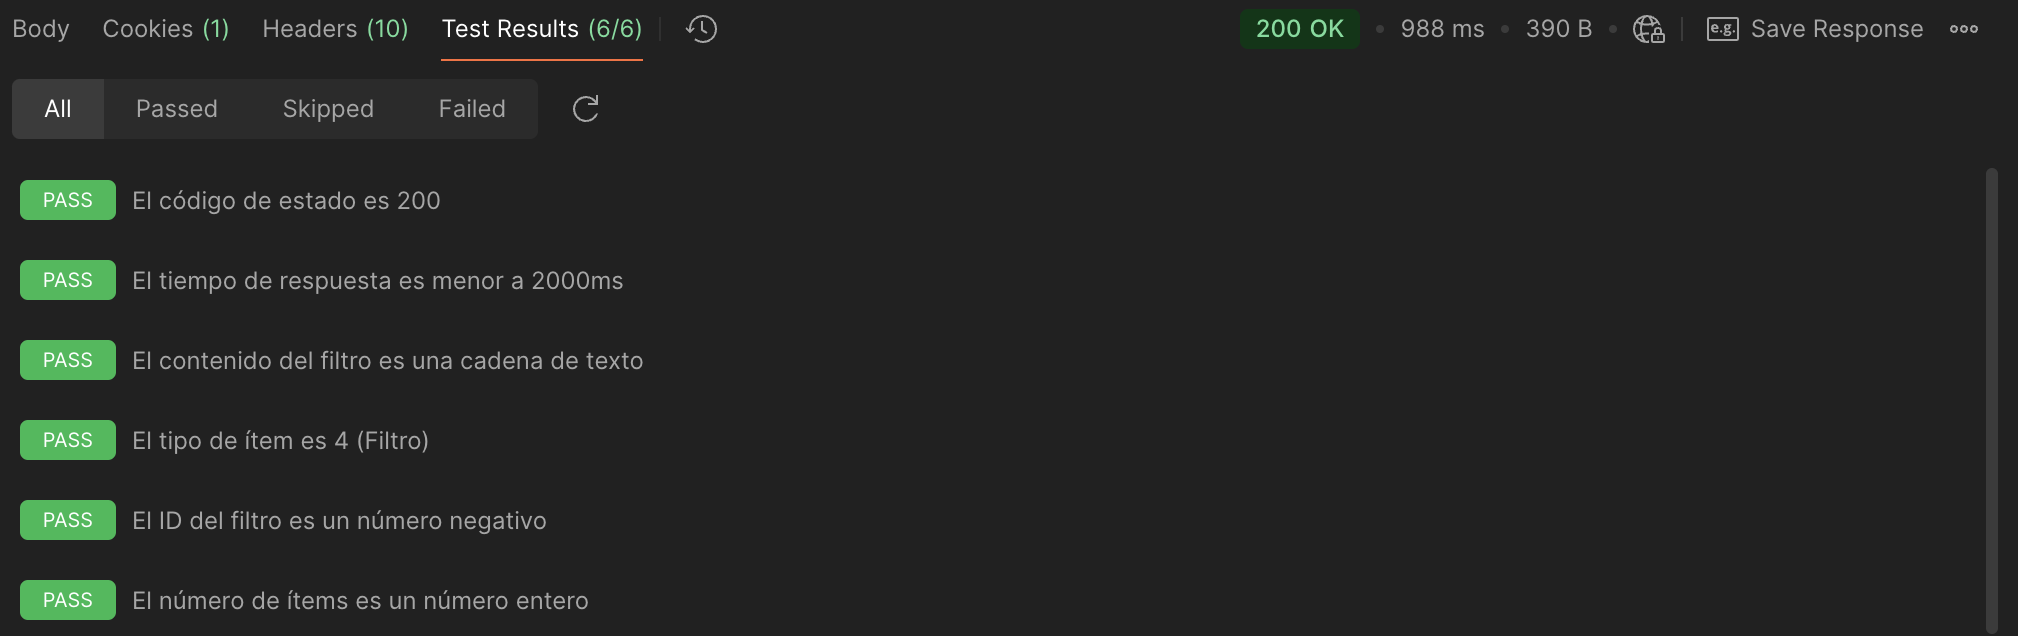
\includegraphics[width=0.9\textwidth]{./imgs/tc1postman.png}
    \caption{Resultado de la prueba GET /Filters/Id en Postman}
    \label{fig:tc1postman} 
\end{figure}


\subsection{GET /Filters/Id/Items}
Este endpoint devuelve la lista de ítems asociados a un filtro específico. Las validaciones incluyen:
\begin{itemize}
    \item Código de estado 200 \checkmark
    \item Tiempo de respuesta menor a 2000 ms \checkmark
    \item La respuesta es una lista de ítems \checkmark
    \item Cada ítem tiene un OwnerId igual a \{\{user\_id\}\} $\checkmark$
    \item Cada ítem tiene un ID válido \checkmark
\end{itemize}

Este endpoint es útil para listar las tareas filtradas por un criterio específico, como las tareas que deben realizarse hoy. Las pruebas aseguran que cada ítem en la lista esté correctamente asociado al usuario autenticado.

\begin{lstlisting}
pm.test("El código de estado es 200", function () {
    pm.response.to.have.status(200);
});

pm.test("El tiempo de respuesta es menor a 2000ms", function () {
    pm.expect(pm.response.responseTime).to.be.below(2000);
});

pm.test("La respuesta es una lista de ítems", function () {
    var jsonData = pm.response.json();
    pm.expect(jsonData).to.be.an('array');
});

pm.test("Verificar que cada ítem tenga el OwnerId igual a {{user_id}}", function () {
    var jsonData = pm.response.json();
    var userId = pm.variables.get("user_id");
    jsonData.forEach(function(item) {
        pm.expect(item.OwnerId).to.eqls(parseInt(userId));
    });
});

pm.test("Verificar que cada ítem tenga un ID válido", function () {
    var jsonData = pm.response.json();
    jsonData.forEach(function(item) {
        pm.expect(item.Id).to.be.a('number').and.to.be.above(0);
    });
});
\end{lstlisting}

\begin{figure}[h!]
    \centering
    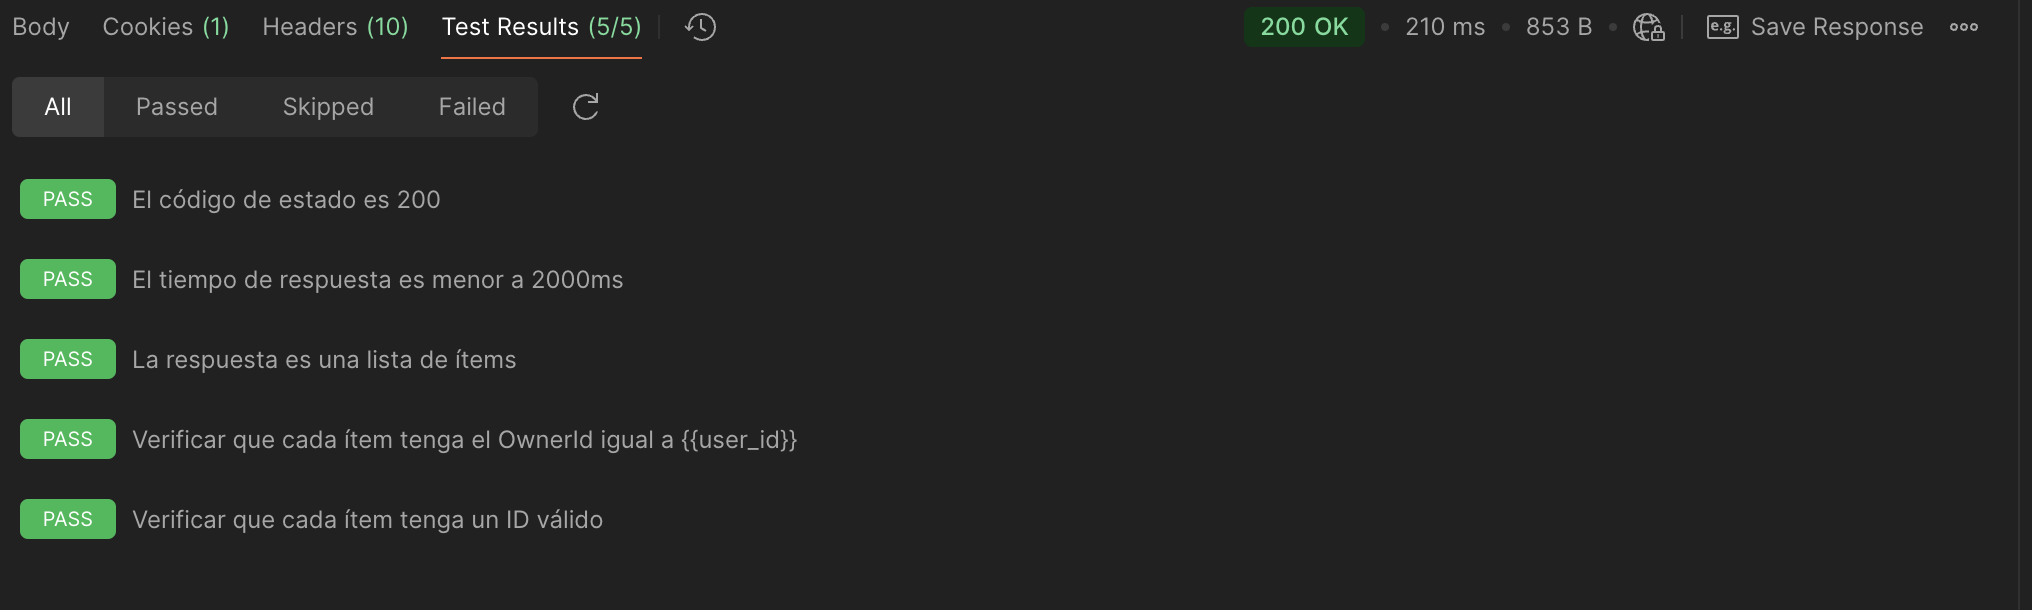
\includegraphics[width=0.9\textwidth]{./imgs/tc2postman.png}
    \caption{Resultado de la prueba GET /Filters/Id/Items en Postman}
    \label{fig:tc2postman}
\end{figure}

\subsection{GET /Filters/Id/DoneItems}
Este endpoint devuelve la lista de ítems completados asociados a un filtro específico. Las validaciones realizadas fueron:
\begin{itemize}
    \item Código de estado 200 \checkmark
    \item Tiempo de respuesta menor a 2000 ms \checkmark
    \item La respuesta es una lista de ítems completados \checkmark
    \item Cada ítem tiene un OwnerId igual a \{\{user\_id\}\} $\checkmark$
    \item Cada ítem tiene un ID válido \checkmark
    \item Verificar que los ítems estén marcados como completados \checkmark
\end{itemize}

Este endpoint permite al usuario ver las tareas que ha completado. Las pruebas aseguran que todos los ítems devueltos estén efectivamente marcados como completados y asociados al usuario correcto.

\begin{lstlisting}
pm.test("El código de estado es 200", function () {
    pm.response.to.have.status(200);
});

pm.test("El tiempo de respuesta es menor a 2000ms", function () {
    pm.expect(pm.response.responseTime).to.be.below(2000);
});

pm.test("La respuesta es una lista de ítems completados", function () {
    var jsonData = pm.response.json();
    pm.expect(jsonData).to.be.an('array');
});

pm.test("Verificar que cada ítem tenga el OwnerId igual a {{user_id}}", function () {
    var jsonData = pm.response.json();
    var userId = pm.variables.get("user_id");
    jsonData.forEach(function(item) {
        pm.expect(item.OwnerId).to.eqls(parseInt(userId));
    });
});

pm.test("Verificar que cada ítem tenga un ID válido", function () {
    var jsonData = pm.response.json();
    jsonData.forEach(function(item) {
        pm.expect(item.Id).to.be.a('number').and.to.be.above(0);
    });
});

pm.test("Verificar ítems completados", function () {
    var jsonData = pm.response.json();
    jsonData.forEach(function(item) {
        pm.expect(item.Checked).to.eqls(true);
    });
});
\end{lstlisting}

\begin{figure}[h!]
    \centering
    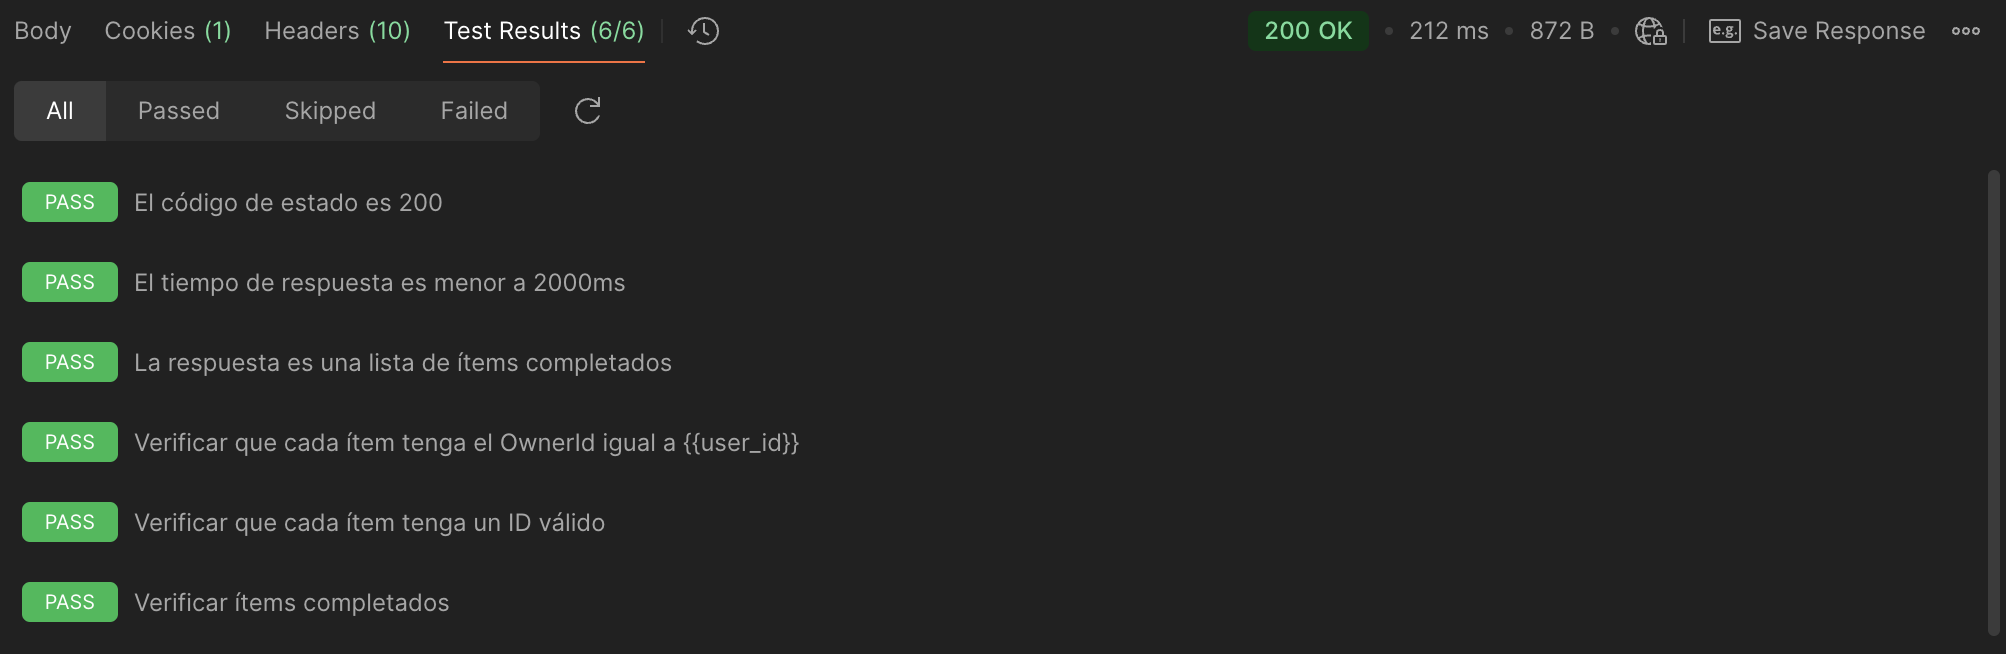
\includegraphics[width=0.9\textwidth]{./imgs/tc3postman.png}
    \caption{Resultado de la prueba GET /Filters/Id/DoneItems en Postman}
    \label{fig:tc3postman}
\end{figure}

\subsection{GET /Items}
Este endpoint devuelve la lista de todos los ítems del usuario autenticado. Las pruebas realizadas fueron:
\begin{itemize}
    \item Código de estado 200 \checkmark
    \item Tiempo de respuesta menor a 2000 ms \checkmark
    \item La respuesta es una lista de ítems \checkmark
    \item Cada ítem tiene un OwnerId igual a \{\{user\_id\}\} $\checkmark$
    \item Cada ítem tiene un ID y contenido válidos \checkmark
\end{itemize}

Este endpoint es fundamental para mostrar todas las tareas de un usuario y comprobar que los datos devueltos sean correctos y completos.

\begin{lstlisting}
pm.test("El código de estado es 200", function () {
    pm.response.to.have.status(200);
});

pm.test("El tiempo de respuesta es menor a 2000ms", function () {
    pm.expect(pm.response.responseTime).to.be.below(2000);
});

pm.test("La respuesta es una lista de ítems", function () {
    var jsonData = pm.response.json();
    pm.expect(jsonData).to.be.an('array');
});

pm.test("Verificar que cada ítem tenga el OwnerId igual a {{user_id}}", function () {
    var jsonData = pm.response.json();
    var userId = pm.variables.get("user_id");
    jsonData.forEach(function(item) {
        pm.expect(item.OwnerId).to.eqls(parseInt(userId));
    });
});

pm.test("Cada ítem tiene un ID y contenido válidos", function () {
    var jsonData = pm.response.json();
    jsonData.forEach(function(item) {
        pm.expect(item.Id).to.be.a('number').and.to.be.above(0);
        pm.expect(item.Content).to.be.a('string').and.to.not.be.empty;
    });
});
\end{lstlisting}

\begin{figure}[h!]
    \centering
    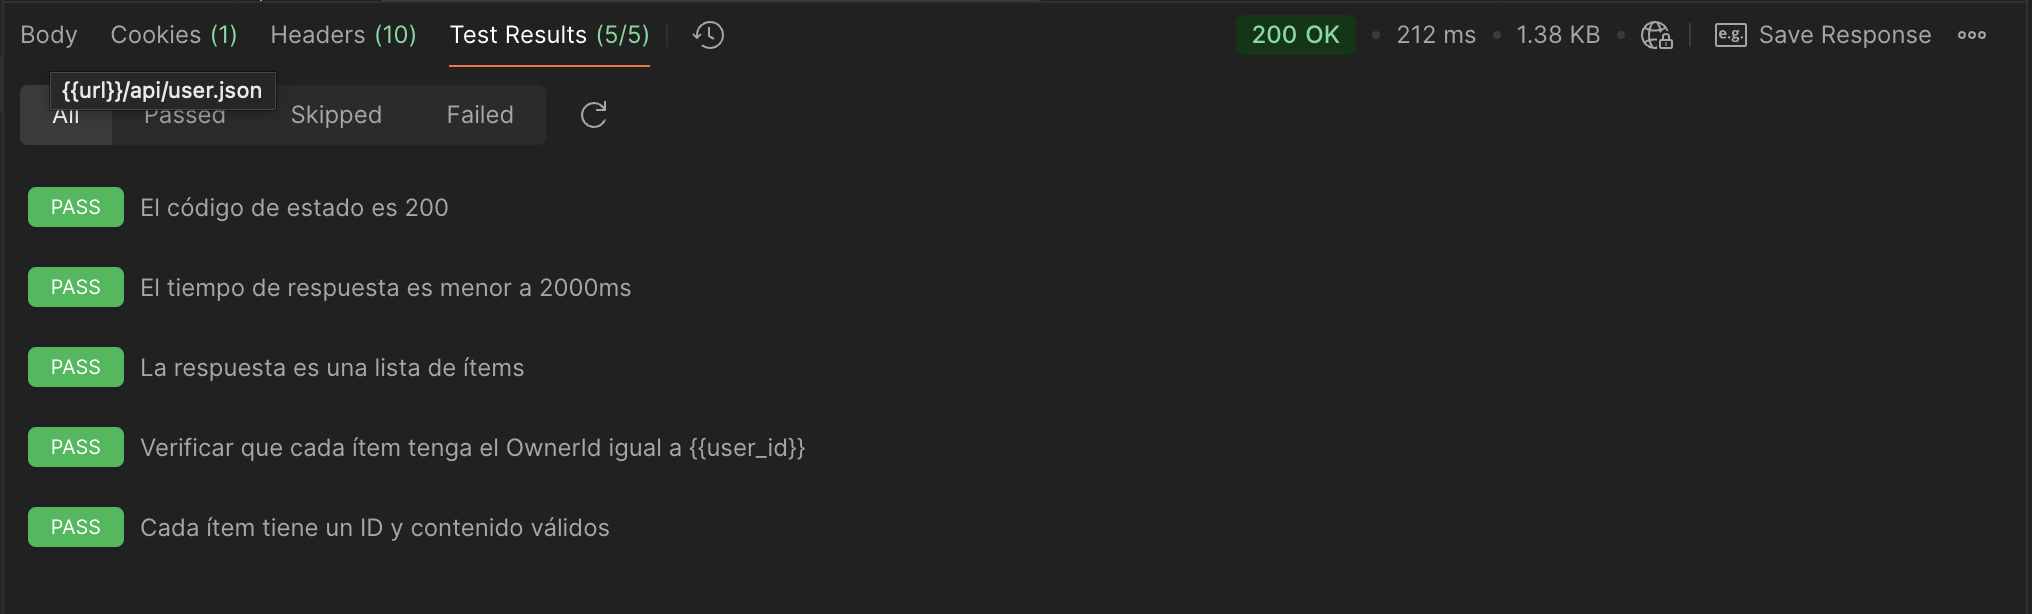
\includegraphics[width=0.9\textwidth]{./imgs/tc4postman.png}
    \caption{Resultado de la prueba GET /Items en Postman}
    \label{fig:tc4postman}
\end{figure}

\section{Conclusión}
El proceso de pruebas de API permitió evaluar la estabilidad, confiabilidad y calidad de los endpoints de Todo.ly, enfocándose en tiempo de respuesta, validez de datos e integridad estructural. Este ejercicio destaca un enfoque sistemático para validar la funcionalidad de una API.

%%%%%%%%%%%%%%%%%%%%%%%%%%%%%%%%%%%%%%%%%%%%%%%%%%%%%%%%%%%%%%%%%%%%%%%%%%%%%%%%
%%
%% Pruebas E2E
%%%%%%%%%%%%%%%%%%%%%%%%%%%%%%%%%%%%%%%%%%%%%%%%%%%%%%%%%%%%%%%%%%%%%%%%%%%%%%%%
\chapter{Pruebas E2E}

Este capítulo aborda las pruebas end-to-end (E2E) diseñadas para verificar flujos completos de usuario en la aplicación Todo.ly. Estas pruebas aseguran que las diferentes funcionalidades trabajen correctamente en conjunto y que el sistema mantenga su integridad durante la interacción con múltiples componentes.

\section{Casos de Prueba E2E}
\begin{figure}[h!]
    \centering
    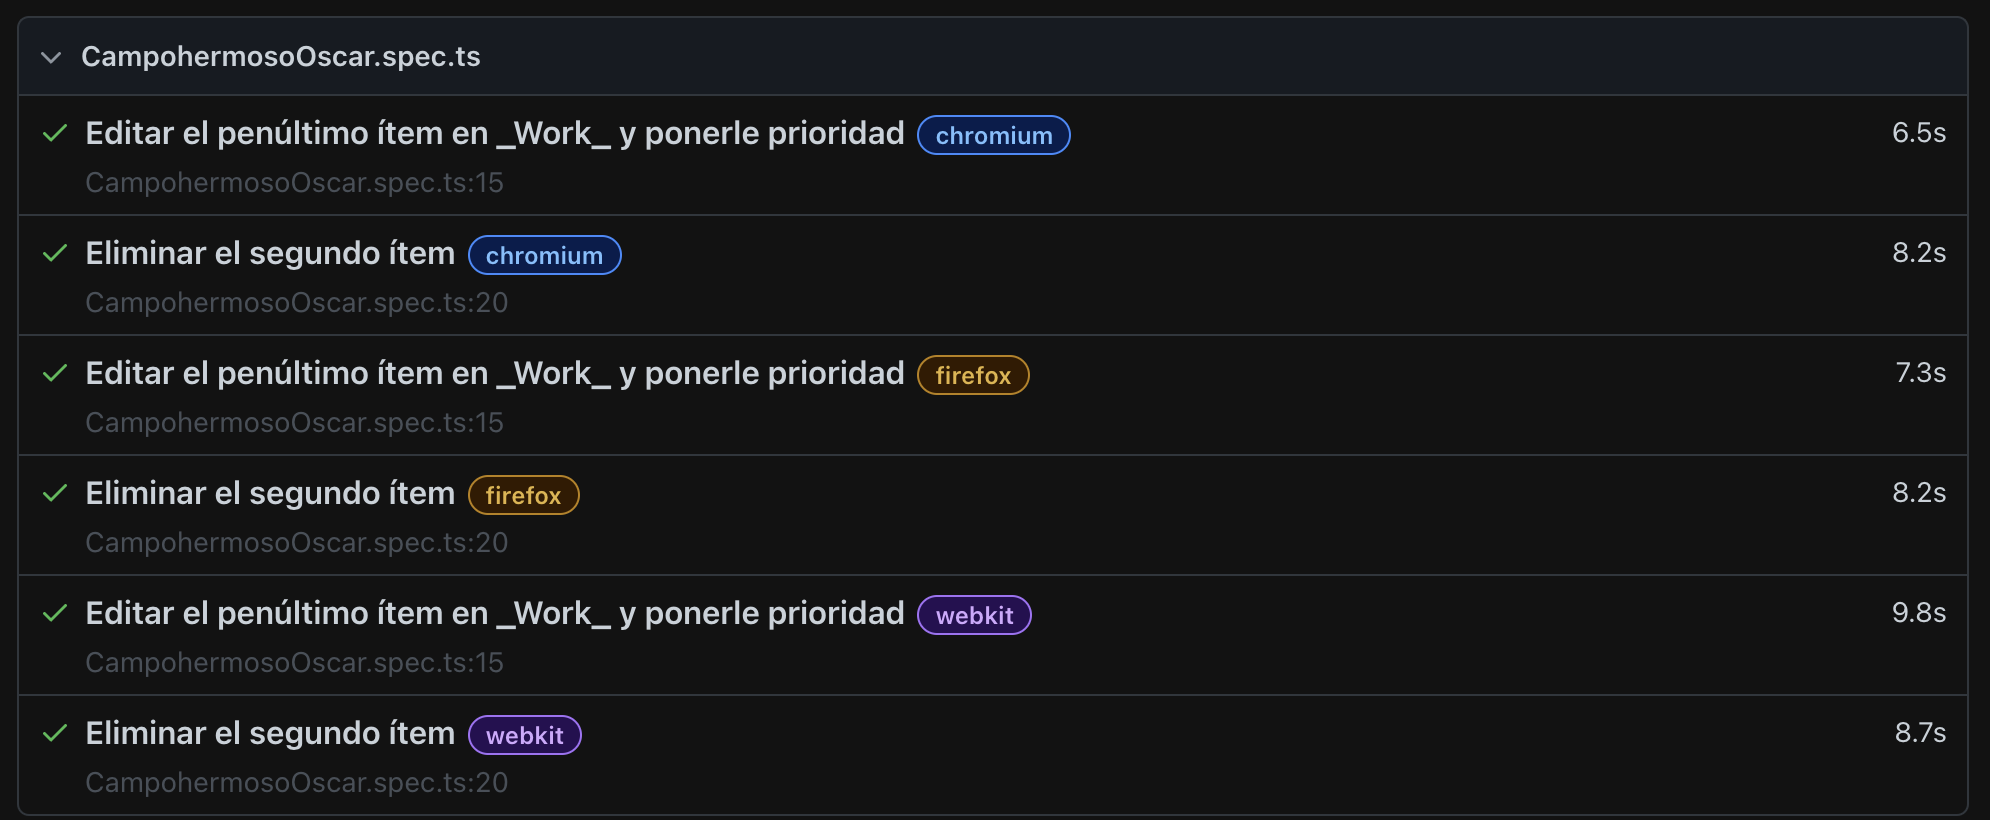
\includegraphics[width=0.9\textwidth]{./imgs/playwright/Captura de pantalla 2024-11-17 a la(s) 21.49.35.png}
    \caption{Reporte de ambas pruebas E2E en Playwright en múltiples navegadores}
    \label{fig:tcsplaywright}
\end{figure}

Se llevaron a cabo dos pruebas en el módulo de tareas de la aplicación Todo.ly. Estas pruebas fueron diseñadas para evaluar la interacción entre las diferentes funciones de la aplicación. A continuación, se describen los casos realizados:

\subsection{Editar el Penúltimo Ítem en \texttt{Work} y Asignarle Prioridad}

Este caso de prueba verifica que un usuario pueda editar una tarea existente dentro del proyecto \texttt{Work}, asignándole prioridad correctamente. Los pasos principales incluyen:
\begin{itemize}
    \item Navegar hasta la lista de tareas en el proyecto \texttt{Work}.
    \item Seleccionar el penúltimo ítem.
    \item Abrir el menú de opciones.
    \item Asignar la prioridad esperada al ítem.
\end{itemize}

La prueba asegura que el cambio de prioridad se refleje visualmente mediante un cambio de color en la tarea editada. A continuación, el código de la prueba:

\begin{lstlisting}
    async openPenultimateTodoItemPriorityMenu() {
        await this.penultimateTodoItemLI.hover();
        await this.penultimateTodoItemMoreOptionsButton.click();
        await this.penultimateTodoItemPriorityButton.click();
        await this.loader.waitFor({ state: 'hidden' });

        // Esperar a que el color cambie a 'rgb(22, 139, 184)'
        await expect(this.penultimateTodoItemLI.locator('.ItemContentDiv'))
        .toHaveCSS('color', 'rgb(22, 139, 184)');
    }
\end{lstlisting}
\begin{figure}[h!]
    \centering
    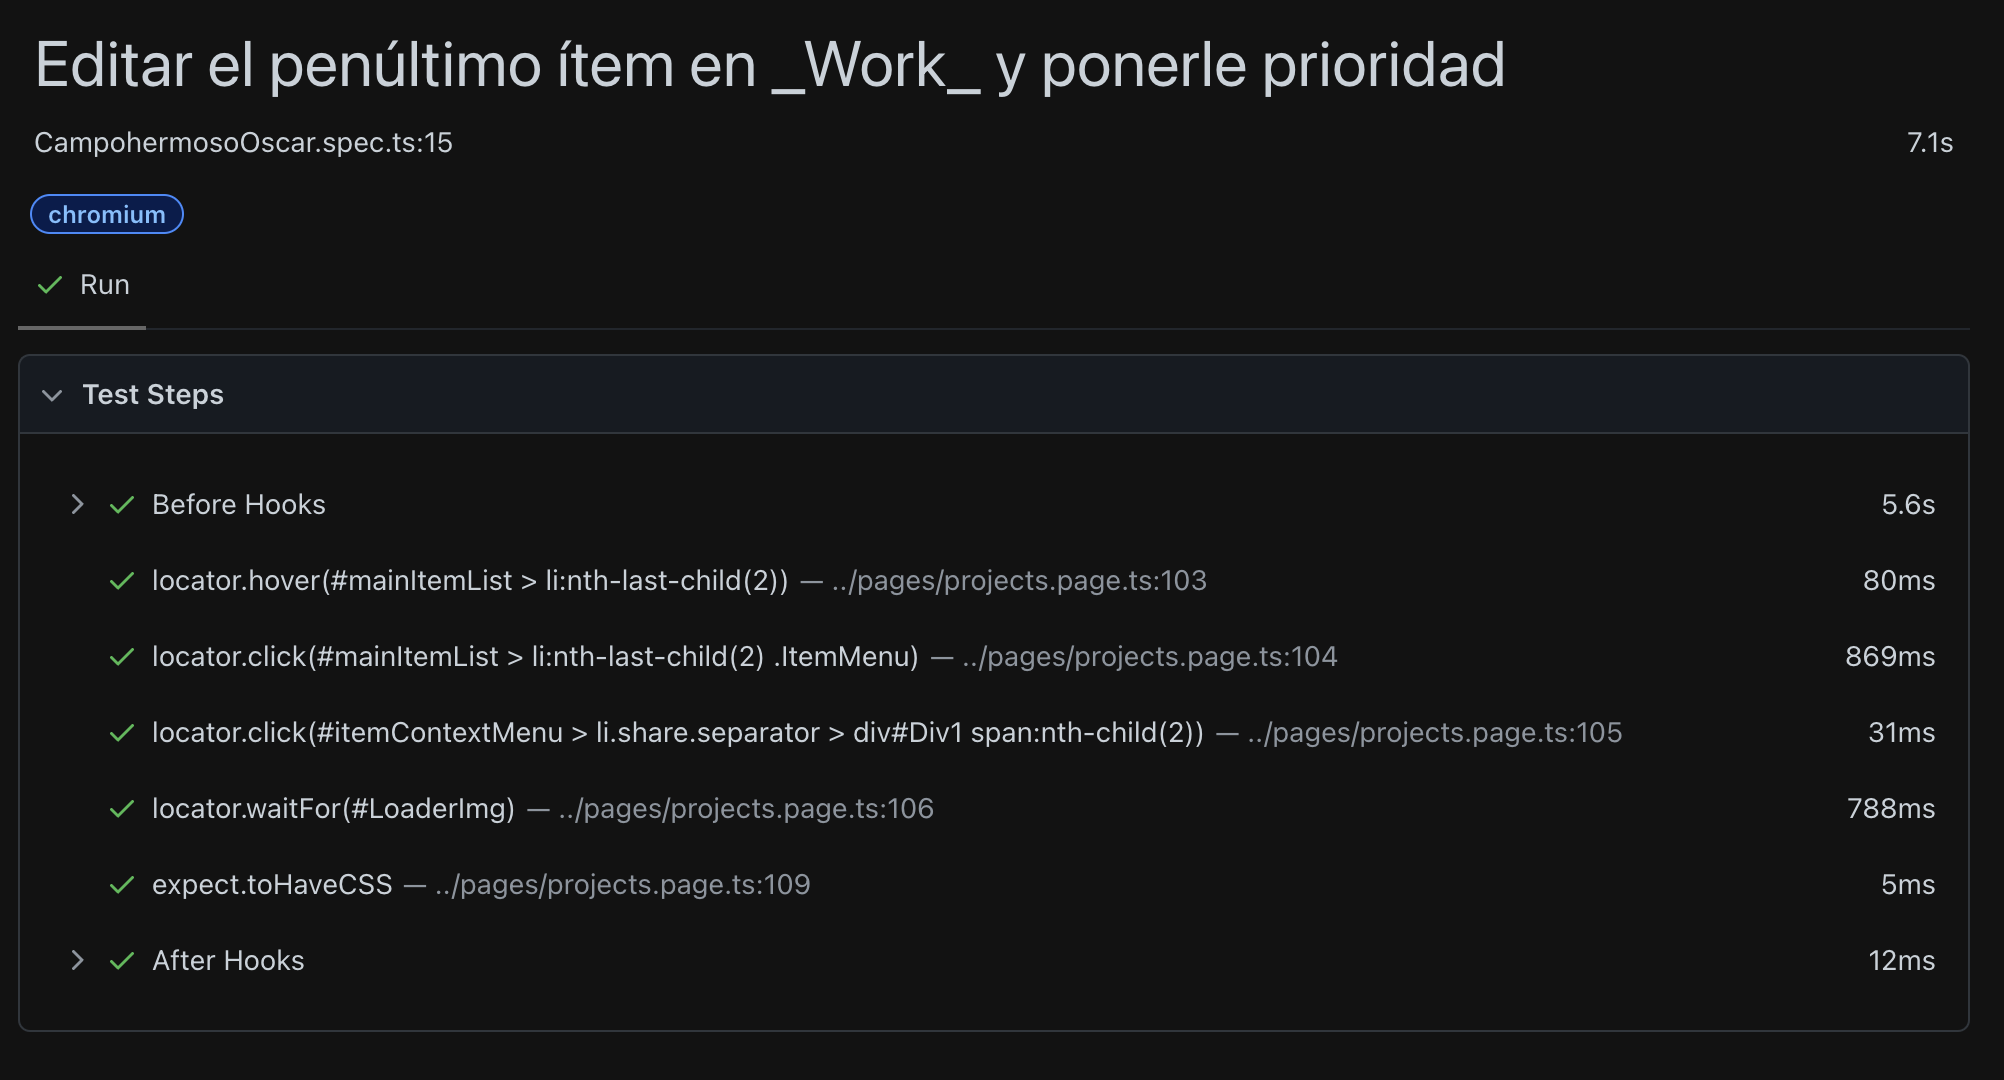
\includegraphics[width=0.8\textwidth]{./imgs/Captura de pantalla 2024-11-19 a la(s) 12.23.05.png}
    \caption{Resumen de los pasos de la prueba en Playwright, realizados en chromium}
    \label{fig:tc1playwright}
\end{figure}

\subsection{Eliminar el Segundo Ítem}

Este caso de prueba valida que un usuario pueda eliminar correctamente una tarea específica, en este caso el segundo ítem de la lista de tareas. Los pasos principales incluyen:
\begin{itemize}
    \item Navegar hasta la lista de tareas.
    \item Seleccionar el segundo ítem.
    \item Abrir el menú de opciones.
    \item Eliminar la tarea seleccionada.
\end{itemize}

La prueba asegura que el ítem eliminado desaparezca de la lista y que no mantenga atributos residuales en el sistema. También valida que el mensaje de confirmación se muestre correctamente y que el proceso de eliminación sea manejado sin problemas incluso si involucra múltiples apariciones del cargador (\texttt{loader}). A continuación, el código de la prueba:

\begin{lstlisting}
    async deleteSecondTodoItem() {
        const itemIdOfSecondTodoItem = await this.secondTodoItemLI.getAttribute('itemid');
    
        if (itemIdOfSecondTodoItem === null) {
            throw new Error('Second todo item does not have an itemid attribute');
        }
    
        await this.secondTodoItemLI.hover();
        await this.secondTodoItemMoreOptionsButton.click();
        await this.secondTodoItemDeleteButton.click();
    
        // Wait for the info message to appear
        await this.messageInfo.waitFor({ state: 'visible' });
    
        // Assert the message content
        await expect(this.messageInfo).toHaveText('Info. Item has been Deleted');
    
        // Wait for the loader to disappear (second appearance)
        await this.loader.waitFor({ state: 'hidden' });
    
        // Ensure the item is no longer in the list
        await expect(this.mainContentTasks).not.toContainText(itemIdOfSecondTodoItem);
    }
\end{lstlisting}
\begin{figure}[h!]
    \centering
    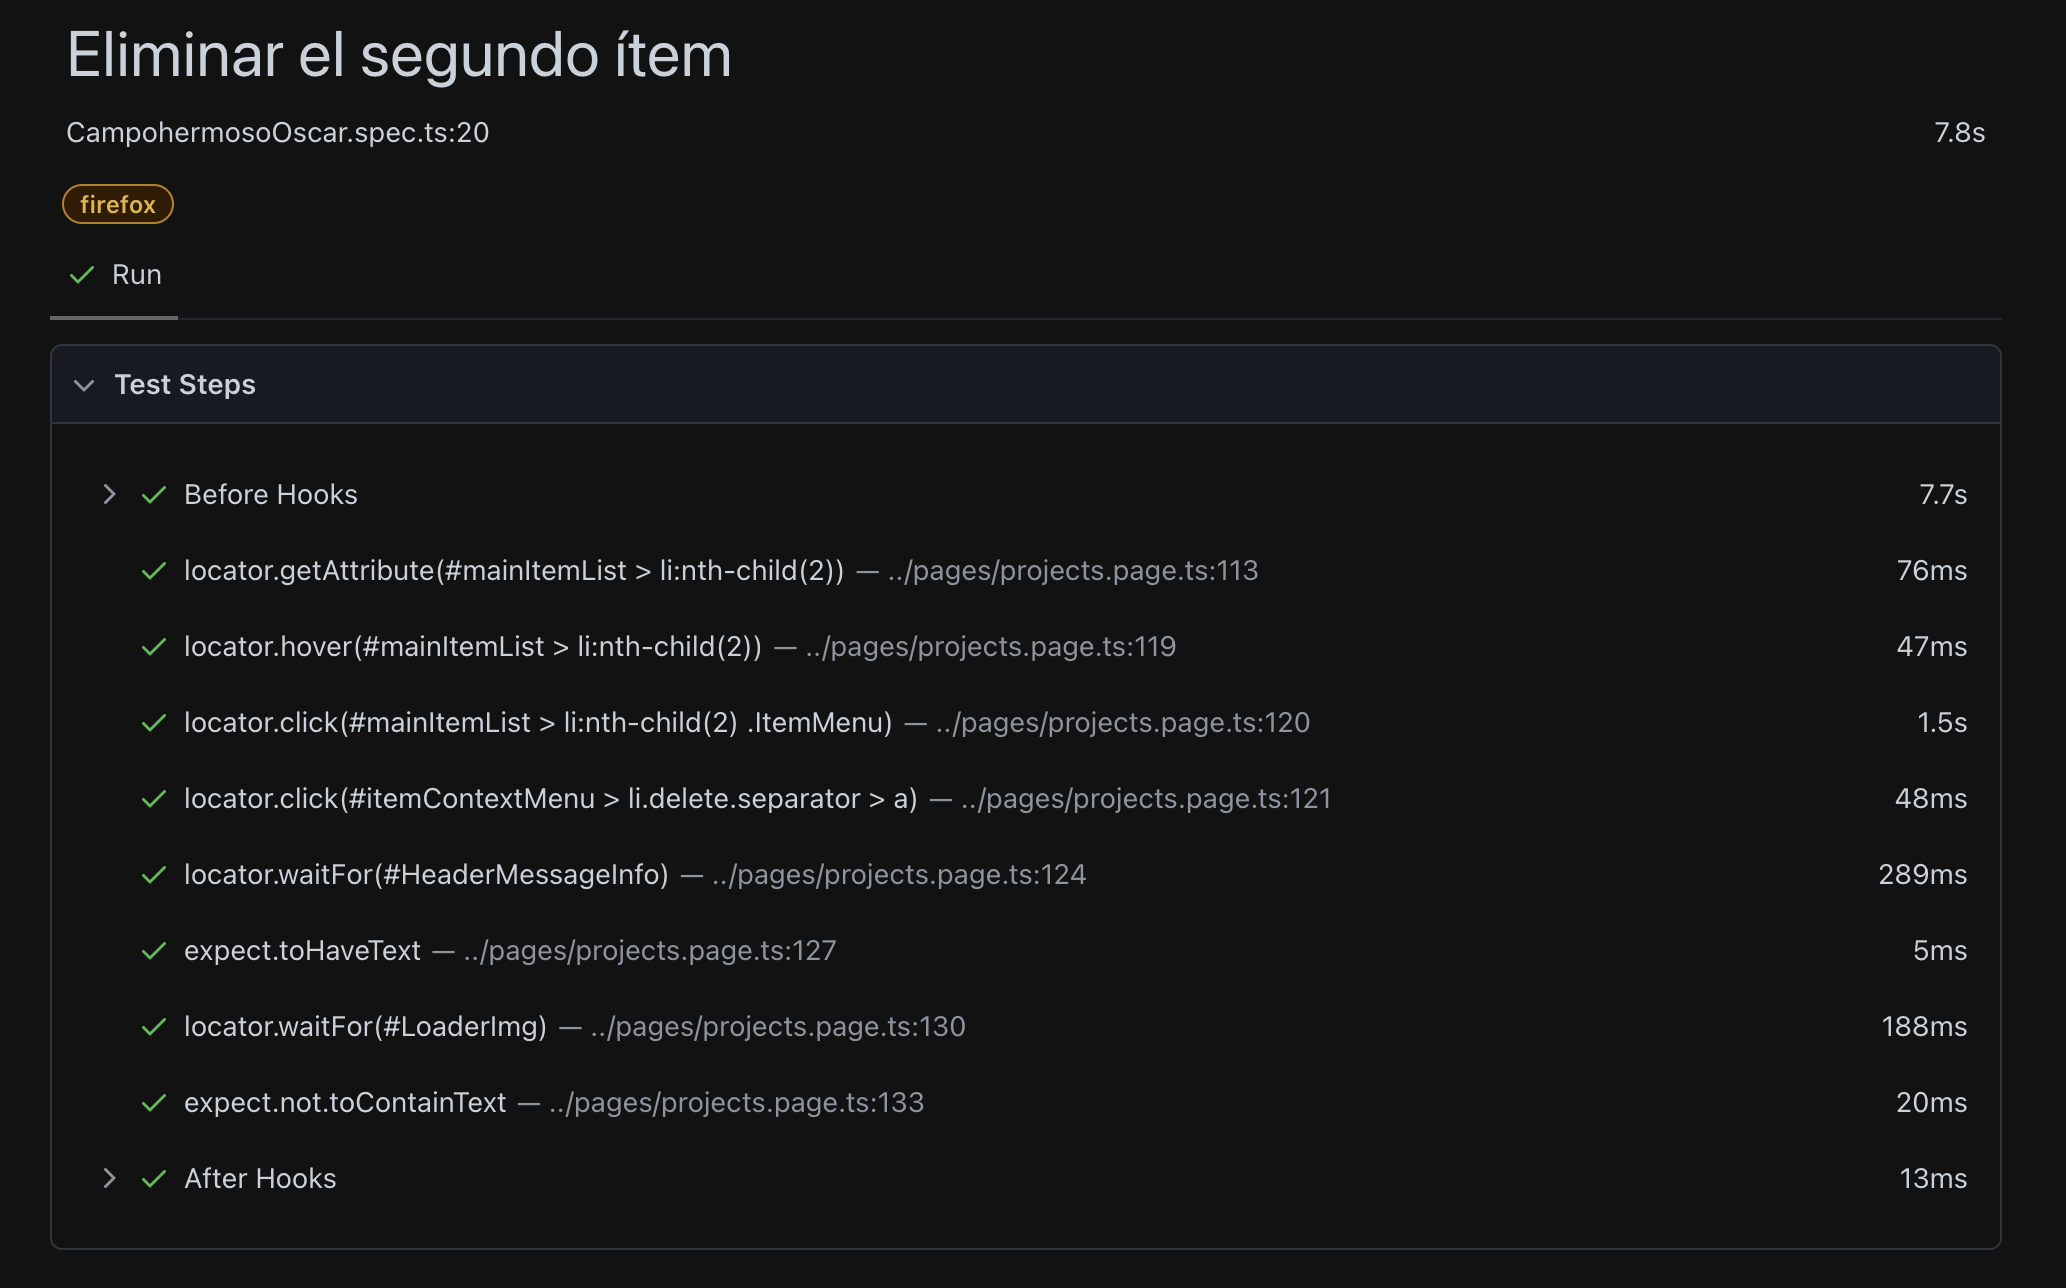
\includegraphics[width=0.7\textwidth]{./imgs/Captura de pantalla 2024-11-19 a la(s) 12.23.18.png}
    \caption{Resumen de los pasos de la prueba en Playwright, realizados en firefox}
    \label{fig:tc2playwright}
\end{figure}

\section{Conclusión}

Las pruebas E2E realizadas demuestran que las funcionalidades clave de Todo.ly operan correctamente en conjunto. Estas pruebas confirman que las tareas pueden ser editadas y eliminadas de manera efectiva, asegurando que los cambios realizados por el usuario se reflejen consistentemente en la interfaz. Además, se validó que el flujo de eliminación maneja correctamente las transiciones entre el mensaje de confirmación y el cargador. La implementación de Playwright permitió automatizar los casos de prueba, optimizando su ejecución y validación.


%%%%%%%%%%%%%%%%%%%%%%%%%%%%%%%%%%%%%%%%%%%%%%%%%%%%%%%%%%%%%%%%%%%%%%%%%%%%%%%%
%%
%% Anexos
%%%%%%%%%%%%%%%%%%%%%%%%%%%%%%%%%%%%%%%%%%%%%%%%%%%%%%%%%%%%%%%%%%%%%%%%%%%%%%%%
\chapter{Anexos}

En esta sección se incluyen recursos adicionales relevantes para la implementación, ejecución y análisis de las pruebas de API y pruebas E2E en la aplicación Todo.ly.

\section{Repositorio de Gestión de Calidad}

El repositorio asociado a este trabajo contiene la implementación de las pruebas realizadas en Postman en formato json, así como documentación en formato \LaTeX{}.

\begin{itemize}
    \item \href{https://github.com/OscarCampohermoso/gestion-calidad-3er-parcial.git}{\texttt{https://github.com/OscarCampohermoso/gestion-calidad-3er-parcial.git}}
\end{itemize}

\section{Repositorio de Pruebas E2E con Playwright}

Este repositorio incluye el código y configuración necesarios para ejecutar las pruebas E2E en la aplicación Todo.ly utilizando Playwright. Contiene scripts, documentación técnica y configuraciones útiles para replicar el entorno de pruebas. Está disponible en el siguiente enlace:

\begin{itemize}
    \item \href{https://github.com/CarrascoAlejandro/CALI_TodoLy_Playwright.git}{\texttt{https://github.com/CarrascoAlejandro/CALI\_TodoLy\_Playwright.git}}
\end{itemize}

\section{Instrucciones para Clonar y Ejecutar los Repositorios}

A continuación, se describen los pasos básicos para clonar y ejecutar los repositorios mencionados:

\subsection{Clonar Repositorios}
Ejecute los siguientes comandos en su terminal para clonar los repositorios:
\begin{verbatim}
# Clonar el repositorio de gestión de calidad
git clone https://github.com/OscarCampohermoso/gestion-calidad-3er-parcial.git

# Clonar el repositorio de pruebas E2E
git clone https://github.com/CarrascoAlejandro/CALI_TodoLy_Playwright.git
\end{verbatim}

\subsection{Ejecución de Pruebas en Playwright}
1. Instalar las dependencias necesarias:
\begin{verbatim}
npm install
\end{verbatim}

2. Ejecutar las pruebas:
\begin{verbatim}
npx playwright test
\end{verbatim}

\subsection{Ejecución de Pruebas de API con Newman}
1. Instalar las dependencias necesarias:
\begin{verbatim}
npm install -g newman
\end{verbatim}

2. Ejecutar las colecciones de Postman:
\begin{verbatim}
newman run API-testing-OscarCampohermoso.postman_collection.json \
-e QAenv-OscarCampohermoso.postman_environment.json --color off
\end{verbatim}

\end{document} 